\section{RAPid-Learn}
\label{sec:rapid_learn_method}

RAPid-Learn (Learning to Recover and Plan Again) solves the executor discovery problem (\cref{def:edp}) by instantiating a targeted reinforcement learning problem for each failed operator and exploiting the agent's symbolic knowledge to guide exploration. This section describes the framework in detail: the overall planning-execution-recovery loop, the construction of the learning problem for failed operators, and the knowledge-guided exploration strategies that make learning sample-efficient.

\subsection{Overview}
\label{sec:rl_overview}

The RAPid-Learn framework operates as follows. The agent begins with an integrated planning task $\IPT = \langle \PlanningTask, M, \Abstraction, e \rangle$ and uses a symbolic planner (MetricFF~\citep{hoffmann2003metricff}) to generate a plan $\Plan = [\Operator_1, \ldots, \Operator_n]$. It then executes this plan operator by operator, using the executor mapping $e$ to realize each operator in the environment. If all executors succeed, the agent reaches its goal. If an executor $e(\Operator_i)$ fails---detected by observing that $\Abstraction(s) \not\models \Eff_{\Operator_i}$ after execution---the agent enters the \emph{executor discovery} phase.

During executor discovery, the agent checks whether it has previously learned an executor for the failed operator. If so, it executes the learned executor directly. If not, it instantiates a reinforcement learning problem focused on achieving the effects of the failed operator and learns a new executor through interaction with the environment. Once a successful executor is learned, it is stored for future use, and the agent resumes execution of the original plan.

This process is summarized in \cref{alg:rapid_learn} and illustrated concretely in \cref{fig:running_example_overview}. The framework handles multiple novelties naturally: if several operators fail (either simultaneously or sequentially), the agent learns a separate executor for each, building up a library of recovery behaviors over time.

\begin{algorithm}[t]
\caption{RAPid-Learn}
\label{alg:rapid_learn}
\begin{algorithmic}[1]
\REQUIRE Stretch-IPT $\tilde{\IPT} = \langle \PlanningTask', M', \Abstraction, e' \rangle$
\STATE $\Plan \gets \text{Planner}(\PlanningTask')$ \COMMENT{$\Plan = [\Operator_1, \ldots, \Operator_{|\Plan|}]$}
\STATE $\Executors \gets \{e(\Operator_i) : \Operator_i \in \Plan\}$
\FOR{$\Operator_i \in \Plan$}
    \STATE $\textit{success} \gets \text{Execute}(e(\Operator_i))$
    \IF{$\neg\,\textit{success}$}
        \IF{$\Executor'_i \in \Executors$}
            \STATE Execute($\Executor'_i$)
        \ELSE
            \STATE $\Executor'_i \gets \text{Discover-Executor}(\Operator_i, \Plan, \tilde{\IPT})$
            \STATE $\Executors \gets \Executors \cup \{\Executor'_i\}$
            \STATE Execute($\Executor'_i$)
        \ENDIF
    \ENDIF
\ENDFOR
\end{algorithmic}
\end{algorithm}

\begin{figure}[t]
    \centering
    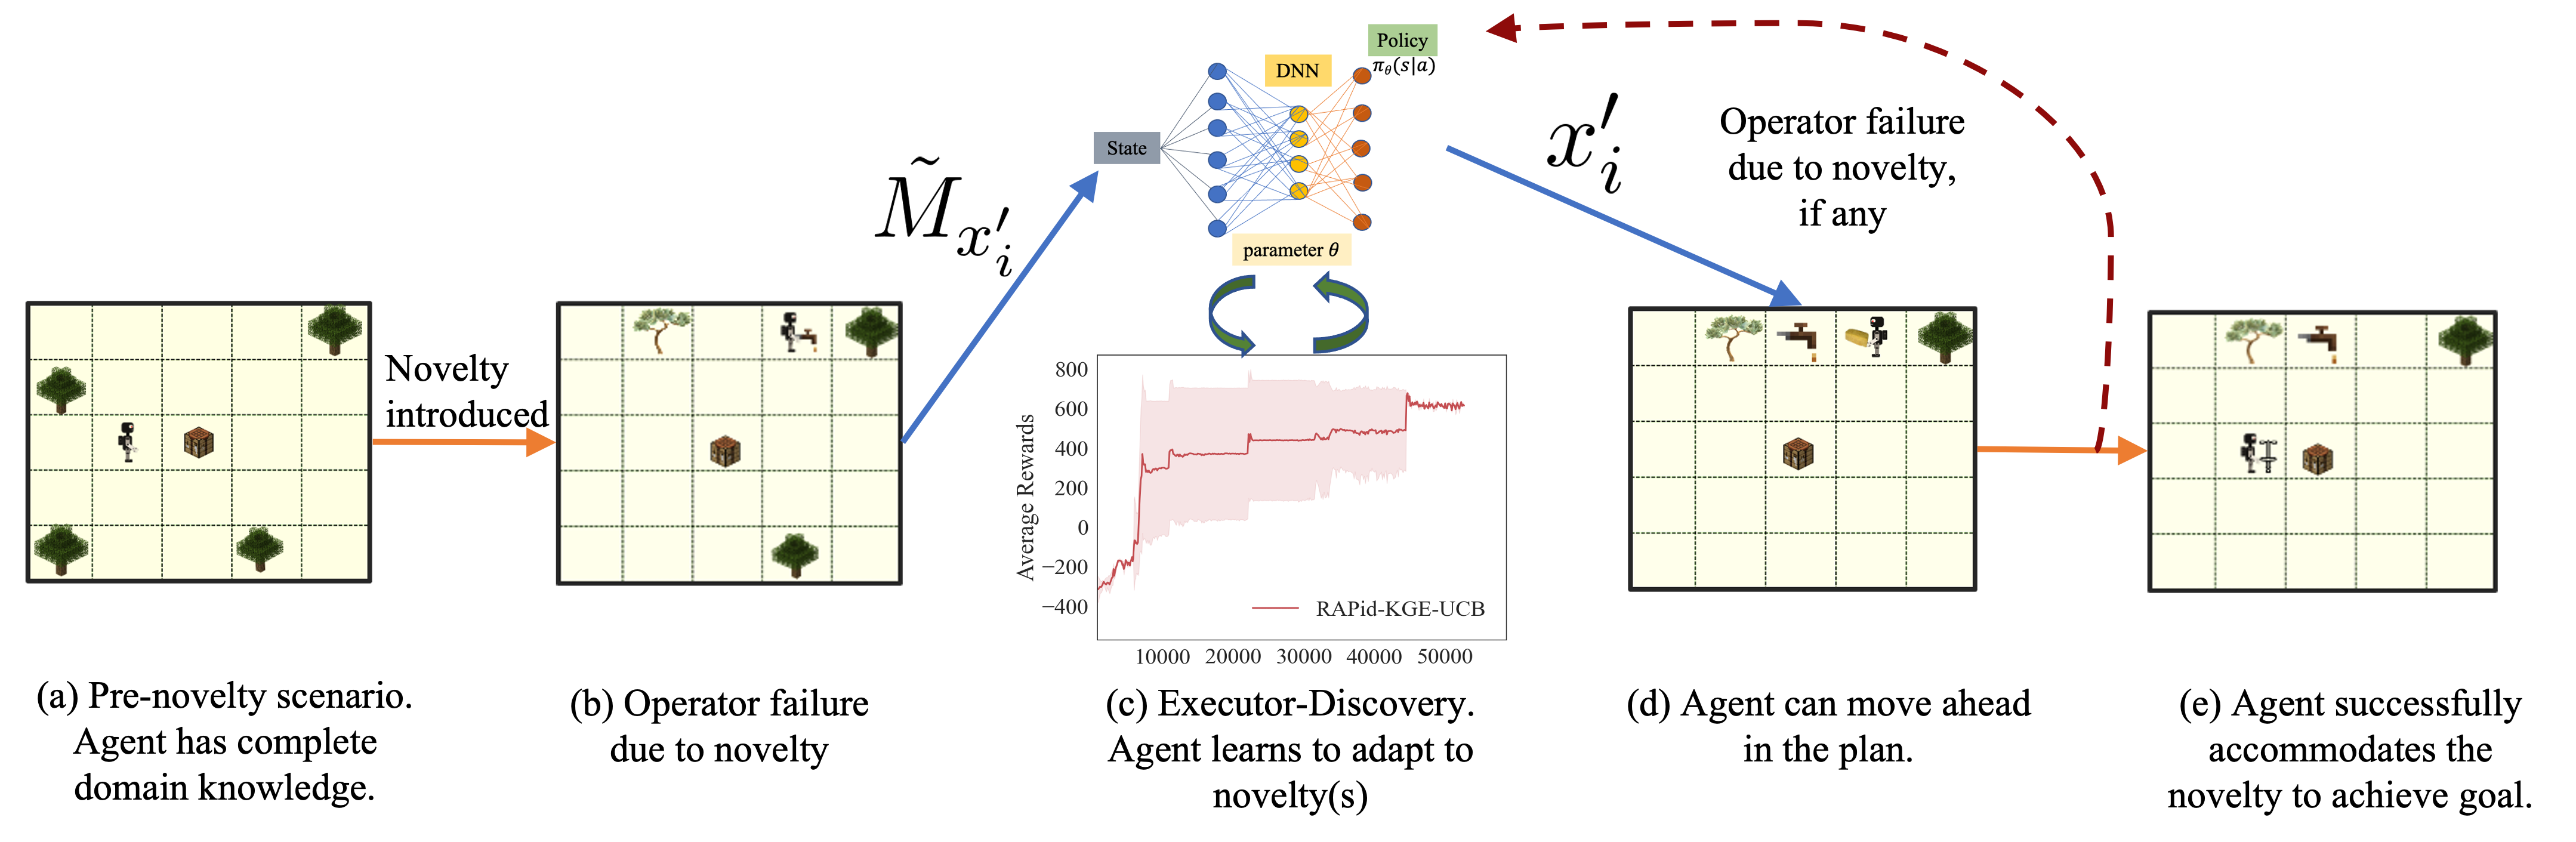
\includegraphics[width=\textwidth]{figures/chapter4/running_example_overview.png}
    \caption{Running example overview of RAPid-Learn under the axe-to-break novelty. The agent detects an execution failure when the \texttt{break} operator does not produce the expected effects. The executor discovery phase instantiates a focused reinforcement learning problem, using knowledge-guided exploration to learn a new executor that first collects the axe and then breaks the tree. Once the executor converges, it is stored and the agent resumes executing the original plan to reach its goal.}
    \label{fig:running_example_overview}
\end{figure}


\subsection{Executor Discovery}
\label{sec:executor_discovery_method}

When operator $\Operator_i$ fails during plan execution, the agent instantiates a reinforcement learning problem to discover a new executor $\Executor'_i$. This involves three components: defining the MDP for the failed operator, generating the set of \emph{plannable states} that serve as success criteria, and designing the reward function.

\paragraph{MDP construction.} For the failed operator $\Operator_i$, the agent constructs an episodic MDP $M_{\Executor'_i} = \langle \States', \Actions', \Transition', \Reward_{\Executor'_i}, \Discount \rangle$, where $\States'$ is the set of environment states, and $\Actions'$ consists of three types of actions: (1) the agent's pre-novelty low-level actions, (2) any novel actions detected in the environment, and (3) higher-level actions corresponding to existing executors (e.g., \texttt{approach} operators that use the internal planner for navigation). Including existing executors as actions in the MDP allows the learner to compose known behaviors with new ones, significantly reducing the exploration space. Each episode begins by executing the plan from the initial state up to the point of failure, so the learner always starts from the state in which the operator failed.

\paragraph{Plannable state generation.} The agent uses its symbolic knowledge to compute the set of \emph{plannable states} $S_r \subseteq \SymStates$---symbolic states from which the agent can generate a valid plan to the goal. These are the target states for the learned executor. The plannable states are computed from the plan $\Plan$ and the failed operator $\Operator_i$ as follows:
\begin{enumerate}[leftmargin=*]
    \item States that satisfy the effects $\Eff_{\Operator_i}$ of the failed operator (the direct recovery case).
    \item States that satisfy the effects $\Eff_{\hat{\Operator}}$ of all subsequent operators $\hat{\Operator} \in \hat{\Operators}$ whose preconditions depend on the effects of $\Operator_i$ (the skip-ahead case, allowing the agent to bypass the failed operator entirely if an alternative path exists).
\end{enumerate}
Formally, $S_r = \{ \SymState : \SymState \models \Eff_{\Operator_i} \} \cup \{ \SymState : \SymState \models \Eff_{\hat{\Operator}} \text{ for all } \hat{\Operator} \in \hat{\Operators} \}$, where $\hat{\Operators}$ is defined as in \cref{sec:ipt_def}. The disjunctive structure of $S_r$ provides the learner with multiple possible recovery targets, increasing the likelihood of finding a viable solution.

\paragraph{Reward function.} The reward function is designed to guide the agent toward plannable states while penalizing irreversible actions. At each time step, the agent receives:
\[
\Reward_{\Executor'_i}(S_r, s, a, s') =
\begin{cases}
+\phi_1 & \text{if } \Abstraction(s') \in S_r \text{ and } \exists \hat{\Plan} \text{ from } \Abstraction(s') \text{ to } \Goal, \\
-\phi_2 & \text{if } \Abstraction(s') \in S_r \text{ and } \nexists \hat{\Plan} \text{ from } \Abstraction(s') \text{ to } \Goal, \\
-1 & \text{otherwise},
\end{cases}
\]
where $\phi_1, \phi_2 > 0$ are reward constants. The first case provides a large positive reward when the agent reaches a plannable state from which the goal is reachable. The second case penalizes reaching a state that appears plannable symbolically but from which no valid plan exists---this can occur when the agent takes irreversible actions during exploration (e.g., using up a limited resource). The third case provides a small step penalty to encourage efficient solutions. Crucially, each time the agent reaches a state in $S_r$, the symbolic planner is invoked to verify that a plan to the goal exists, ensuring that the learned executor actually resolves the impasse.


\subsection{Knowledge-Guided Exploration}
\label{sec:kge}

A na\"ive reinforcement learning agent exploring the post-novelty environment would face a large state-action space with a sparse reward signal, leading to slow convergence. RAPid-Learn addresses this through \emph{knowledge-guided exploration}: using the agent's symbolic domain knowledge to focus exploration on states and actions that are likely relevant to the novelty. Two complementary strategies are employed.

\paragraph{Knowledge-guided curriculum learning.} Complex novelties may require the agent to first reach a promising region of the state space before meaningful exploration can begin. With probability $\rho$ at the start of each episode, the agent is provided with a curriculum: a novel entity $\epsilon \in \Entities'$ is selected, and the symbolic planner is used to generate a plan that brings the agent to the vicinity of that entity. The agent then begins its reinforcement learning exploration from this more informative starting state. This strategy leverages the insight that novelties are typically associated with new entities or changed objects in the environment, and that reaching those entities is a prerequisite for discovering recovery behaviors.

\paragraph{Knowledge-guided action biasing.} During exploration, the agent biases its action selection toward a subset of actions $\Delta$ that are likely relevant to the novelty. This subset consists of (1) novel actions that appeared in the environment after the novelty, and (2) the failed operator itself (in executor form), since retrying it in different states or with different preconditions satisfied may succeed. Two methods for action biasing are developed:

\emph{Upper Confidence Bound biasing (KGE-UCB).} With probability $\epsilon_0$, the selection probability of each action $a' \in \Actions'$ is modified as:
\[
\hat{\Policy}(a') \gets \Policy(a') + 
\begin{cases}
+c \sqrt{\frac{\ln t}{N_t(a')}} & \text{if } a' \in \Delta, \\[6pt]
-c \sqrt{\frac{\ln t}{N_t(a')}} & \text{if } a' \notin \Delta,
\end{cases}
\]
where $c > 0$ is an exploration constant, $t$ is the current time step, and $N_t(a')$ is the number of times action $a'$ has been selected up to time $t$. This formulation, inspired by the Upper Confidence Bound algorithm~\citep{auer2002ucb}, encourages the agent to try actions in $\Delta$ that have been attempted the least, systematically exploring novel actions while gradually reducing exploration of familiar ones.

\emph{Uniform action biasing (KGE-UAB).} An alternative strategy that uniformly increases the probability of selecting actions in $\Delta$ by a multiplicative factor $\mu > 1$:
\[
\hat{\Policy}(a') \gets 
\begin{cases}
\frac{(\mu - 1 + \sum_\Delta) \cdot \Policy(a')}{\mu \sum_\Delta} & \text{if } a' \in \Delta, \\[6pt]
\frac{\Policy(a')}{\mu} & \text{if } a' \notin \Delta,
\end{cases}
\]
where $\sum_\Delta = \sum_{a \in \Delta} \Policy(a)$ is the total probability mass assigned to actions in $\Delta$ under the current policy.

Both methods are extensions of $\epsilon$-greedy exploration that incorporate domain knowledge about which actions are most likely to be relevant for resolving the novelty. The rationale follows from two assumptions: (1) the agent should exploit its existing domain knowledge to direct exploration rather than exploring uniformly, and (2) the novelty that caused the impasse is likely related to novel entities or actions in the environment.

\subsection{Recovery and Executor Reuse}
\label{sec:recovery}

The agent trains its policy using a policy gradient algorithm~\citep{williams1992reinforce} and monitors convergence through a success rate criterion: if the agent achieves the positive reward (reaching a plannable state with a valid plan to the goal) in at least $\eta$ out of the last $n$ episodes, the policy is considered converged. The learned policy $\Policy^c_{\Executor'_i}$ is then encapsulated as a new executor:
\[
\Executor'_i = \langle S'_0, \Policy^c_{\Executor'_i}, \beta_{\Executor'_i} \rangle,
\]
where $S'_0$ is the set of states from which the executor was trained (the failure states), and $\beta_{\Executor'_i}$ is the termination condition derived from the plannable states $S_r$ (as defined in \cref{sec:ipt_def}).

The learned executor is added to the agent's executor set $\Executors$ and mapped to the failed operator. On subsequent encounters with the same failure, the agent executes the stored executor directly without relearning, amortizing the cost of exploration over future episodes. This mechanism is effective even when multiple operators fail: each failure triggers an independent executor discovery process, and the resulting executors are composed through the original symbolic plan structure. The framework naturally handles three types of multiple-operator failures:
\begin{itemize}[leftmargin=*]
    \item \emph{Independent failures}: Multiple novelties cause different operators to fail independently. The agent learns a separate executor for each.
    \item \emph{Cascading failures}: The learned executor for one failure inadvertently causes a downstream operator to fail. The agent detects the new failure and learns an additional executor.
    \item \emph{Simultaneous failures}: Multiple operators fail in the same plan execution. The agent addresses them sequentially as they are encountered during plan execution.
\end{itemize}